% !TeX root = main.tex
\markboth{}{} % remove previous chapter header from blank page before chapter start
\chapter{Research Methodology}\label{Chap:2}
A short summary of the chapter.
\section{Purpose and Aim}

\noindent Some introductory text \ref{fig:sora1}.

\begin{figure}[H]
	\centering
	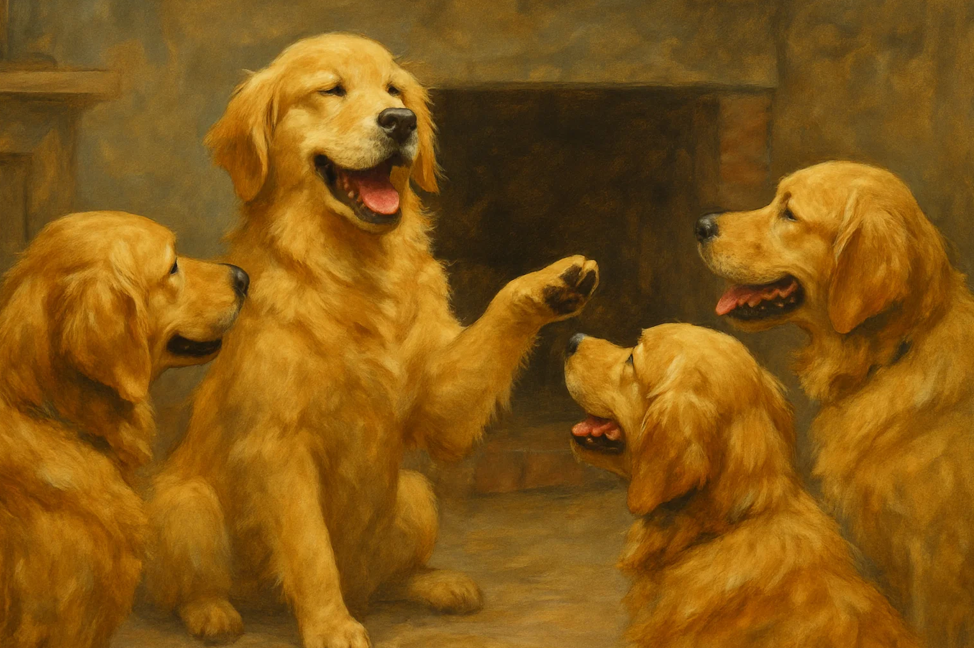
\includegraphics[scale=0.45]{graphics/Picture_1.png}
	\caption{Image generated by Sora \cite{einstein1935can}.}
	\label{fig:sora1}
\end{figure}

\noindent More introductory text.\\
 As an example, see Fig. \ref{fig:sora2}b.

\begin{figure}[H]
	\centering
	\begin{subfigure}{0.5\linewidth}
		\centering
		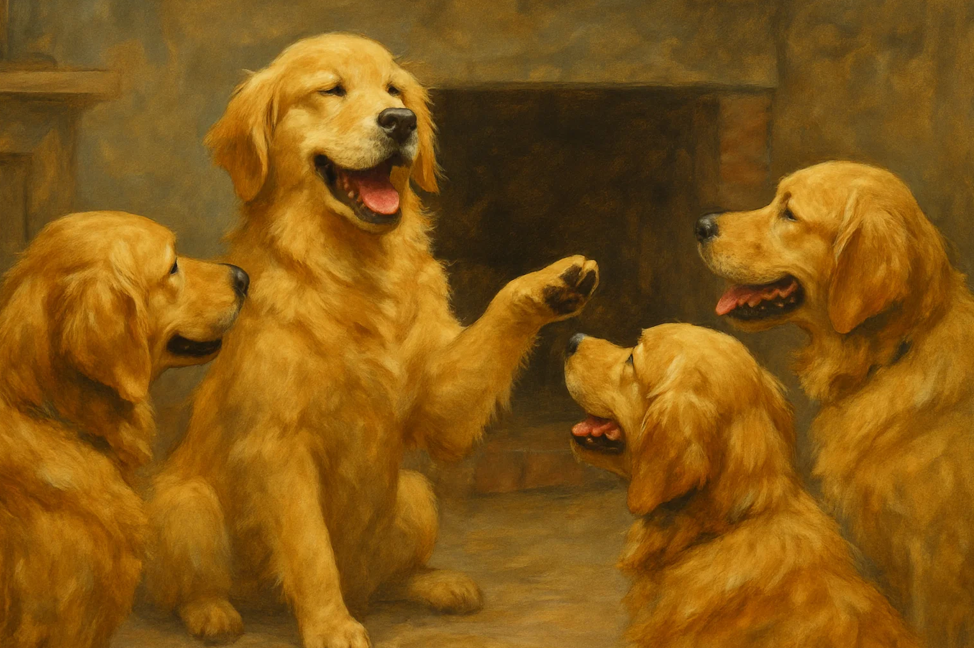
\includegraphics[scale=0.2]{graphics/Picture_1.png}		
		\caption{Dogs.}
		\vspace{-3pt}
		\label{fig:iron-mech}
	\end{subfigure}%
	\begin{subfigure}{0.5\linewidth}
		\centering
		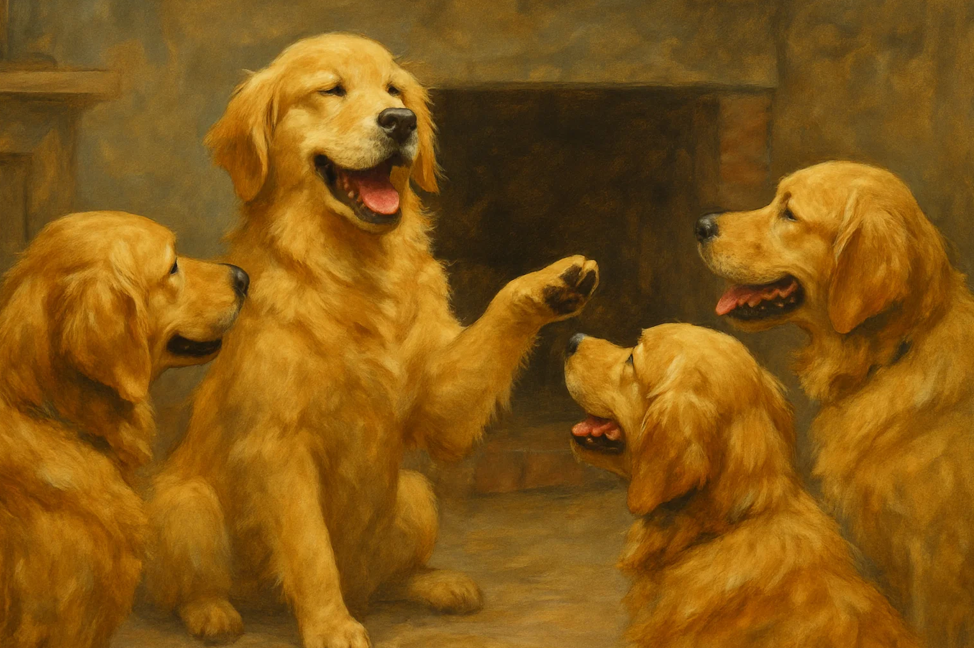
\includegraphics[scale=0.2]{graphics/Picture_1.png}		
		\caption{Same Dogs.}
		\vspace{-3pt}
		\label{fig:iron-phys}
	\end{subfigure}
	\caption{Image generated by Sora \cite{einstein1935can}.}
	\label{fig:sora2}
\end{figure}


\section{Research Design}\label{sec:2.2}

\noindent Outline your research design here.\\ 

\section{Materials and Methods}

\noindent Outline your Materials and Methods here. Don't forget to be very thorough, and, above all, clear about the limitations of your setup and methods.\\

\subsection{Of course you can also do subsections}
\subsubsection{And sub sub.} 
